\chapter{Introduction}
\label{cha:introduction}

\section{Macroscopic City Movements - problem definition}
\label{cha:introduction_probdef}

\textbf{Here we should describe what problem project is about to solve. In the 1st term presentation I mentioned that we want to answer two questions:
}\\
 
Given a location, where and in what proportion people move to another location - Movement Graph? 
\\
Where and how long do people stay at certain location? - but we need to be more precise here.

\section{Localization-based services and positioning technologies}
\label{cha:introduction_methodo}

TODO: we need here more details about what our Sudanian guy were supposed to research
\subsection{Positioning technologies}

TODO: http://geoawesomeness.com/knowledge-base/location-based-services/location-based-services-technologies/

\subsection{Localization-based services}

\textbf{We should describe what are proactive and reactive LBS- https://www.move-forward.com/gps-everywhere-location-based-services/. Here we should describe how the data is obtained, and emphasise the fact that location updates are based on MOVEMENTS, so each next point is triggered by some mobile phone movement. Point updates are not triggered while being stationary. }

\begin{figure}[!ht]
	\centering
	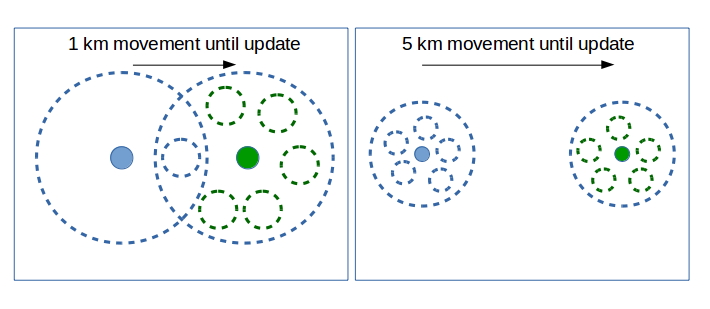
\includegraphics[width=0.9\textwidth]{images/movement_update.png}\\
	\caption{Continuous and Discontinuous location update after movement to section lacking area details  }
	\label{fig:movement_update}
\end{figure}
\FloatBarrier

Because of the characteristics of GPS and other localization methods, in so called urban canyons and the like, signal loss with re–acquisition times of 45 seconds to five minutes can be observed. This could lead to discontinuous recording of the location - \autoref{fig:movement_update}
